\documentclass[bachelor,zhspacing]{cqu}  %单面打印版本
\usepackage{etex}
\def\tightlist{}

%%在这增加你需要的其它包
\definecolor{hellgelb}{rgb}{1,1,0.8}
\definecolor{colKeys}{rgb}{0,0,1}
\definecolor{colIdentifier}{rgb}{0,0,0}
\definecolor{colComments}{rgb}{1,0,0}
\definecolor{colString}{rgb}{0,0.5,0}
\usepackage{listings}
\lstset{%
    float=hbp,%
    basicstyle=\ttfamily\small, %
    identifierstyle=\color{colIdentifier}, %
    keywordstyle=\color{colKeys}, %
    stringstyle=\color{colString}, %
    commentstyle=\color{colComments}, %
    columns=flexible, %
    tabsize=4, %
    frame=single, %
    extendedchars=true, %
    showspaces=false, %
    showstringspaces=false, %
    numbers=left, %
    numberstyle=\tiny, %
    breaklines=true, %
   backgroundcolor=\color{hellgelb}, %
    breakautoindent=true, %
    captionpos=b,%
	xleftmargin=0pt%
}

\begin{document}

%-----------------------------------论文题目-------------------------------------------------
\xuehao{20121892}
\cntitle{重庆大学\LaTeX 学位论文模板CQU使用说明}
\cnauthor{张乐}
\cnmajor{软件工程}
\cnteacher{葛永新}
\cnxueyuan{软件学院}
\entitle{An Instruction of the \LaTeX\ Templet for Chongqing University Thesis}
\enauthor{Le Zhang}
\enmajor{Software Engineering}
\enteacher{Prof. Yongxin Ge}
\enxueyuan{College of Software}
\cnkind{****}
\enkind{****}
%\cnzlteacher{ }  %%助理教师,如果必要,还要将cqu.cls中的有关该项前的%号去掉
%\enzlteacher{ }
\cndate{二O一六年六月}
\endate{June 2016}
%%%%只需修改上面的相关信息%%%%%%%%
\makecntitle 
\makeentitle 
%%%%%%%%%%%%%%%%%%%%%%%%%%%

\pagenumbering{Roman}
\setcounter{page}{0}
%------------------------------------文章摘要------------------------------------------------------------
\cnkeywords{模板,摘要,论文,\LaTeX}
\begin{cnabstract}
摘要是设计或论文内容不加注释和评论的简短陈述,应以第三人称陈述。它应具有独立性和自含性,
即不阅读设计或论文的全文,就能获得必要的信息,摘要的内容应包含与设计或论文同等量的主要信
息,供读者确定有无必要阅读全文,也供文摘等二次文献采用。\par
摘要一般应说明研究工作目的、实验研究方法、结果和最终结论等,而重点是结果和结论。摘要中一
般不用图、表、化学结构式、计算机程序,不用非公知公用的符号、术语和非法定的计量单位。\par
摘要页置于英文题名页后。 \par
中文摘要一般为400汉字左右,用小四号宋体。 \par
关键词是为了文献标引工作从设计(论文)中选取出来用以表示全文主题内容信息款目的单词或术
语。一般每篇设计(论文)应选取3~5个词作为关键词,关键词间用逗号隔开,最后一个词后不打标点
符号。以显著的字符排在同种语言摘要的下方。如有可能,尽量用《汉语主题词表》等词表提供的规
范词。\par
本文介绍重庆大学论文模板cqu的使用方法。本模板符合学校的本科论文格式基本要求,而硕博模板
有待完善。
本文的创新点主要有:
\begin{itemize*}
\item 用例子来解释模板的使用方法;
\item 用废话来填充无关紧要的部分;
\item 一边学习摸索一边编写新代码。
\end{itemize*}
(模板作者注:中文关键词定义cnkeywords应在使用中文摘要环境之前。英文关键词同理。)
\end{cnabstract} 
\enkeywords{template, \LaTeX, abstract, paper}
\begin{enabstract}
     An abstract of a dissertation is a summary and extraction of 
research work and contributions. Included in an abstract should be 
description of research topic and research objective, brief 
introduction to methodology and research process, and summarization 
of conclusion and contributions of the research. An abstract should be 
characterized by independence and clarity and carry identical 
information with the dissertation. It should be such that the general 
idea and major contributions of the dissertation are conveyed
without reading the dissertation.\par
     An abstract should be concise and to the point. It is a 
misunderstanding to make an abstract an outline of the dissertation and 
words “the first chapter”, “the second chapter” and the like should be 
avoided in the abstract.\par
     Key words are terms used in a dissertation for indexing, 
reflecting core information of the dissertation. An abstract may 
contain a maximum of 5 key words, with semicolons used in between to 
separate one another.
\end{enabstract}
%%%%%%%%%%%%%%%%%%%%%%%%%%%%%%%%%%%%%%

%--------------文章目录-------------
\tableofcontents
\listoffigures
%\addcontentsline{toc}{section}{插图清单}
\listoftables
%\addcontentsline{toc}{section}{附表清单}


%------------------------------------词汇------------------------------------------------------------
\begin{denotation}{2.5}{0}

\item[cluster] 集群
\item[Itanium] 安腾
\item[SMP] 对称多处理
\item[API] 应用程序编程接口
\item[PI]   聚酰亚胺
\item[劝  学] 君子曰:学不可以已。青,取之于蓝,而青于蓝;冰,水为之,而寒于水。
  木直中绳。(车柔)以为轮,其曲中规。虽有槁暴,不复挺者,(车柔)使之然也。故木
  受绳则直, 金就砺则利,君子博学而日参省乎己,则知明而行无过矣。吾尝终日而思
  矣,  不如须臾之所学也;吾尝(足齐)而望矣,不如登高之博见也。登高而招,臂非加
  长也,  而见者远;  顺风而呼,  声非加疾也,而闻者彰。假舆马者,非利足也,而致
  千里;假舟楫者,非能水也,而绝江河,  君子生非异也,善假于物也。积土成山,风雨
  兴焉;积水成渊,蛟龙生焉;积善成德,而神明自得,圣心备焉。故不积跬步,无以至千
  里;不积小流,无以成江海。骐骥一跃,不能十步;驽马十驾,功在不舍。锲而舍之,朽
  木不折;  锲而不舍,金石可镂。蚓无爪牙之利,筋骨之强,上食埃土,下饮黄泉,用心
  一也。蟹六跪而二螯,非蛇鳝之穴无可寄托者,用心躁也。\pozhehao{} 荀况
\end{denotation}

%%%%%%%%%%%%%%%%%%%%%%%%%%%%%%%%%%%%%%%

\pagenumbering{arabic}

\section{前言}\label{ux524dux8a00}

\section{相关工作}\label{ux76f8ux5173ux5de5ux4f5c}

\subsection{稀疏表示}\label{ux7a00ux758fux8868ux793a}

信号稀疏表示的最初目的是为了用比香农定理更低的采样率来表示和压缩信号\textsuperscript{{[}1{]}},就像离散余弦变换和小波变换等。在过去几年里,稀疏表示已经被用于很多信号处理,模式识别的实际应用中。例如,在信号的图片处理领域,稀疏表示被用于信号压缩和编码\textsuperscript{{[}2{]}},图片去噪\textsuperscript{{[}3{]}},图片超像素图片超像素\textsuperscript{{[}4{]}}。在模式识别领域,稀疏表示被用于目标识别和分类任务\textsuperscript{{[}5{]}}\textsuperscript{{[}6{]}}。一些研究表明基于稀疏表示的分类器非常有效,在一些人脸数据库上的识别率甚至是目前的最高水平。

正如在离散余弦变换和小波变换中,原始信号可以用基函数表示,稀疏表示则是用一个称之为字典的超完备冗余的函数系统来代替原始基函数,并利用字典\(\mathbf{X}\)中最少的原子来表示一个原始信号\(b\)。

稀疏表示的思想如下\textsuperscript{{[}7{]}}:假设样本集\(X\)有可以分为\(k\)类的共\(m\)个训练样本,\(X_{k} = [x_{k1},x_{k2},\ldots,x_{kl_{k}}]\in R^{n\times l_{k}}\)表示属于第\(k\)类的l个样本集,如果训练样本足够多,则属于第\(k\)类的任意一个样本\(y\in R^{n}\)可以近似地表示成此类的所有训练样本的线性组合
\[\mathbf{y}=h_{k1}\mathbf {x}_{k1}+h_{k2}\mathbf {x}_{k2}+\ldots+h_{kl_{k}}\mathbf {x}_{kl_{k}}\]
目标函数如下: \[\min_{s}\Vert{s}\Vert_{0}\] \[s.t. \quad b=Xs\]
假如有\(\mathbf{N}\)

\subsection{鉴别稀疏保持投影}\label{ux9274ux522bux7a00ux758fux4fddux6301ux6295ux5f71}

稀疏保持投影\textsuperscript{{[}8{]}}将所有样本作为字典原子进行稀疏重构,鉴别稀疏保持投影则是增强了同类数据的稀疏表示权重\textsuperscript{{[}9{]}},在保持局部结构的同时保持样本之间的总体信息,通过局部合并,以整体的方式发现和重建数据集的内在规律。并通过求解最小二乘问题来更新SPP中的稀疏权重矩阵,得到了一个更能真实反映鉴别信息的鉴别稀疏权重。将无监督的SPP转换成有监督的DSPE,充分利用训练样本中的标签信息。
样本训练集\(X=[X_{1},X_{2},\ldots,X_{c}]\),其中,\(X_{i}=[x_{i1}\ldots,X_{ik}]\in \mathbf{R}^{m\times k}\)是类别标记为\(label(i)\)的样本集合,即第\(i\)类样本。通过最小二乘法获得最能反映类别鉴别信息的权重,目标函数如下:
\[\min_{t}\quad\Vert x_{ij} - \mathbf{X}_{i}t\Vert_{2}\]
\[s.t.\quad It = 1\]
其中\(\mathbf{t}=[t_{1},t_{2},\ldots,t_{j-1},0,t_{j+1},\ldots,t_{k}]^{\mathbf{T}}\),第\(j\)个分量为0,即将任一向量利用同类中除自身以外的向量进行表示。经证明\textsuperscript{{[}9{]}},该方法具有良好的鲁棒性,具有旋转、平移、尺度不变的特性。
为了考虑样本集的全局几何结构,DSPE进一步考虑异类样本对原样本重构的影响。将\(\hat{t}\in \mathbf{R}^k\)扩展到\(n\)个分量\(\hat{h}=[\vec{0},\ldots,\vec{0},\hat{t},\vec{0},\ldots,\vec{0}]\in \mathbf{R}^{n}\),即将除鉴别信息权重以外的系数设置为0.令\(er=x_{ij}-X\hat{t}=x_{ij}-X\hat{h}\),对\(er\)进行在超完备字典\(\hat{X}=[X_{1},X_{2},\ldots,X_{c}\)上的稀疏表示,其中\(X_{i}=\vec{0}\),将人脸样本由鉴别信息权重重构后得到的残差有其他类的所有样本进行稀疏重构:
\[\min_{s}\quad\Vert{s}\Vert_{1}\]
\[s.t.\quad\Vert{er-\hat{X}s}\Vert_{1}<\epsilon\] \[Is = 0\]
作如下变换: \[s^{+} = \left\{ 
    \begin{array}{ll}
        s, & s>0\\
        0, & s\le{0}
    \end{array} \right.\] \[s^{-} = \left\{ \begin{array}{ll}
        -s,&s<0\\
        0, &s\ge{0}
        \end{array}\right.\]
由于\(s^{+},s^{-}\)非负,\(s=s^{+}+s^{-}\),\(\Vert{s}\Vert_{1} = \Sigma_{i}(s_{i}^{+}+s_{i}^{-})\),目标函数转化为
\[\min_{s^{+}+s^{-}}\quad\sum_{i}(s_{i}^{+}+s_{i}^{-})\]
\[s.t.\quad \Vert{er-[\hat{X},-\hat{X}][s^{+},s^{-}]^{T}}\Vert < \epsilon\]
\[[I,-I][s^{+},s^{-}]^{T}=0\]
将优化结果\(\hat{s}=[\hat{s_{1}},\ldots,\hat{s_{i-1}},\vec{0},\hat{s_{i+1},\ldots,\hat{s_{c}}}]\)与\(\hat{t}\)串联,得鉴别稀疏权重\(\hat{d}=\hat{s}+\hat{h}=[\hat{s_{1}},\ldots,\hat{s_{i-1}},\hat{t},\hat{s_{i+1}},\ldots,\hat{s_{c}}]\in \mathbf{R}^{n}\)。由于\(I\hat{t}=1\),\(I\hat{s}=1\),故\(I\hat{d}=1\),该鉴别稀疏权重能够保持旋转,平移,尺度不变的特性\textsuperscript{{[}9{]}}与SPP相比较,DSPE中最小化同类样本重构数更加趋近于0,既增强了同类费劲林样本在重构中的作用,又削弱了异类伪近邻样本对原样本重构的影响,有利于保持同类样本相互靠近,异类样本相互远离的本质。当\(er=0\)时,鉴别稀疏权重便退化成了类似于NPE保持低维流形上同类数据近邻关系的重构权重,表明DSPE能很好地反映数据在低维流形上的分布,与此同时,对\(er\)的稀疏表示有利于加强算法的鲁棒性
DSPE的目标在于将数据间的鉴别稀疏重构特征进行保持并嵌入到低维流形上,因此,数学模型如下:
\[\min_{W}\quad\sum_{i=1}^{n}\Vert{W^{T}x_{i}-W^{T}X\hat{d_{i}}}\Vert^{2}\]
\[s.t. W^{T}XX^{T}W=1\] 对目标函数进行变换,目标函数转换成
\[\max_{W}\quad W^{T}XMX^{T}W\] \[s.t.\quad W^{T}XX^{T}W=1\]
其中,\(M=D+D^{T}-D^{T}D\),目标函数可以通过求解广义特征值得解
\[XMX^{T}W=\lambda XX^{T}W\]
选取最大的\(d\)个特征值所对应的特征向量\(\mathbf{a}_{i}\)构成特征子空间,即可得到DSPE的线性降维映射\(W_{DSPE}=[a_{1},a_{2},\ldots,a_{d}].\)
DSPE既反映了样本间的鉴别关系,又能很好地排除伪类样本在重构人脸数据时带来的负面影响,经实验,在多个人脸库上效果超过PCA,LDA,NPE,LPP,SPP等算法。

\subsection{核技巧}\label{ux6838ux6280ux5de7}

\subsubsection{非线性分类问题}\label{ux975eux7ebfux6027ux5206ux7c7bux95eeux9898}

非线性分类问题是指通过利用非线性模型才能很好地进行分类的问题\textsuperscript{{[}10{]}}。如下图所示,左图为一个分类问题,图中``.''表示正实例点,``\(\times\)''表示负实例点

\begin{figure}[htbp]
\centering
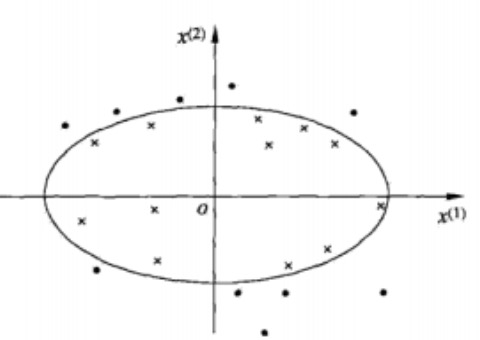
\includegraphics{pic/ellipse.png}
\caption{非线性分类问题与核计巧示例}
\end{figure}

\begin{figure}[H]
  \centering
  \subfloat{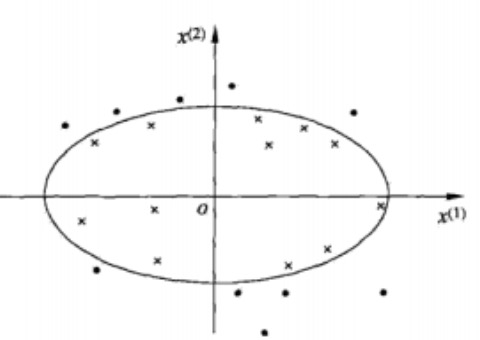
\includegraphics[scale=0.4]{pic/ellipse.png}}\qquad
  \subfloat{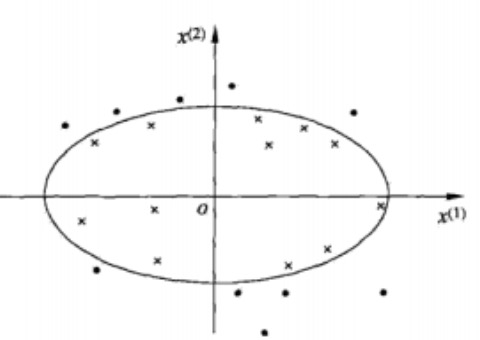
\includegraphics[scale=0.4]{pic/ellipse.png}}
  \caption{含两个子图形的图形}
\end{figure}

在实际分类中,样本本身可能存在线性不可分的情况,而将特征通过非线性映射到高维空间后,往往就可分了。但往往存在确定非线性映射函数的形式和参数、特征空间维数等问题,在进行高维特征空间运算时存在的``维数灾难''问题也是维度转换的一大问题,而核函数则可以有效解决这些问题。

核函数的主要思想如下:设\(\mathbf{x},\mathbf{z}\in\mathbf{X},\mathbf{X}\)属于\(R(n)\)空间,非线性函数\(\phi\)实现输入空间\(\mathbf{X}\)到特征空间\(\mathbf{F}\)的映射,其中\(\mathbf{F}\)属于\(R(m),n\ll m\),且有:
\[\mathbf{K}(\mathbf{x},\mathbf{z}) = <\phi (x),\phi (z)>\]
其中:\(<\mathbf{x},\mathbf{z}>\)为两者内积,\(\mathbf{K}(\mathbf{x},\mathbf{z})\)为核函数。从公式看出核函数可以将\(m\)维高维空间的内积运算转化为\(n\)维低维输入空间的核函数计算,避免了``维数灾难'',减少了计算量。输入空间的维数\(n\)对核函数矩阵无影响,因此可以有效处理高维输入。在进行转换的过程中,我们并不需要知道非线性变换函数\(\phi\)的形式和参数,但核函数的形式和参数的变化会隐式地改变从输入空间到特征空间的映射,对特征空间性质产生影响,最终改变各种核函数的性能。核函数的思想可以和传统的方法相结合,形成多种不同的基于很函数技术的方法,可以为不同的应用选择不同的核函数和算法。目前基于核函数的传统方法改造已取得一些成果,核主成分分析(kernel
PCA)\textsuperscript{{[}11{]}}、核部分最小二乘法(kernel
PLS)\textsuperscript{{[}12{]}}和核\(Fisher\)鉴别分析(Kernel Fisher
Discriminator,KFD)\textsuperscript{{[}13{]}}是核函数的典型用例,在应用中都取得了不错的效果。

\section{核鉴别稀疏保持嵌入}\label{ux6838ux9274ux522bux7a00ux758fux4fddux6301ux5d4cux5165}

\subsection{核鉴别信息权重}\label{ux6838ux9274ux522bux4fe1ux606fux6743ux91cd}

将样本信息\(X_{i}=[x_{i1},\ldots,x_{ik}]\)映射到高维空间为\(B_{i}=[\phi(x_{i1}),\ldots,\phi(x_{ik})]\),只要证明\(\Vert x_{ij}-X_{i}t\Vert\)越小,则\(\Vert \phi(x_{ij})-X_{i}t\Vert\)越小最小二乘问题变为
\[\min_{t}\Vert{\phi{(x_{ij})}-B_{i}t}\Vert_{2}\] \[s.t.\quad It=1\]
因为\(B\)和\(\phi{x}\)是未知的,所以目标函数不能直接求解,所以将问题转化成以下约束:
\[\min_{t}\Vert{B^{T}\phi{(x_{ij})}-B^{T}B_{i}t}\Vert_{2}\]
\[s.t.\quad It=1\] 求证
\(\Vert x_{ij}-X_{i}t\Vert\),\[\min_{t}\Vert{\phi{(x_{ij})}-B_{i}t}\Vert_{2}\],\[\min_{t}\Vert{B^{T}\phi{(x_{ij})}-B^{T}B_{i}t}\Vert_{2}\]同时达到最小值

\[B_{i}^{T}\phi{(x_{ij})}=
        \left[
            \begin{array}{ccc}
                \phi{(x_{i1})}\\
                \phi{(x_{i2})}\\
                \vdots\\
                \phi{(x_{ik})}
            \end{array}
        \right]\phi{(x_{ij})}=
        \left[
            \begin{array}{ccc}
                k(x_{i1},x_{ij})\\
                k(x_{i2},x_{ij})\\
                \vdots\\
                k(x_{ik},x_{ij})
            \end{array}
        \right]\]

\[B_{i}^{T}B_{i}=
    \left[
        \begin{array}{ccc}
            \phi{(x_{i1})}\\
            \phi{(x_{i2})}\\
            \vdots\\
            \phi{(x_{ik})}
        \end{array}
    \right]
    \left[
        \begin{array}{cccc}
            \phi{(x_{i1})} & \phi{(x_{i2})} & \ldots & \phi{(x_{ik})}
        \end{array}
    \right]=
    \left[
        \begin{array}{cccc}
            k(x_{i1},x_{i1}) & k(x_{i1},x_{i2}) & \ldots & k(x_{i1},x_{ij})\\
            k(x_{i2},x_{i1}) & k(x_{i2},x_{i2}) & \ldots & k(x_{i2},x_{ij})\\
            \vdots & \vdots & \ddots & \vdots \\
            k(x_{i3},x_{i1}) & k(x_{i3},x_{i2}) & \ldots & k(x_{i3},x_{ij})
        \end{array}
    \right]\]

目标函数转换成线性规划问题,可以求解。

\subsection{核稀疏重构权重}\label{ux6838ux7a00ux758fux91cdux6784ux6743ux91cd}

令\(C=[\phi{(X_{1})},\phi{(X_{2})},\ldots,\phi{(X_{c})}]\),令\(C_{i}=[\phi{(X_{1})},\ldots,\phi{(X_{i-1})},\phi{(X_{i+1})},\ldots,\phi{(X_{c}})]\)即从超完备字典中剔除样本\(X_{i}\)
令\(er=\phi{(x_{ij})}-B_{i}\hat{t}=\phi{(x_{ij})}-C\hat{h}\),即样本由鉴别信息权重重构后得到的残差,对其对样本中的其他类进行重构:
\[\begin{array}{ll}
        \min_{s} & \Vert{s}\Vert_{1}\\
        \\
        s.t.  & \Vert{er-C_{i}s}\Vert < \epsilon \\
        & Is = 0
    \end{array}\]
同理由于函数\(\phi\)不能直接求解,将\({er-C_{i}s}\)左乘\(C^{T}\)转换成\({C_{i}^{T}(er-C_{i}s)}\),即\(C^{T}\phi{(x_{ij})}-C^{T}C\hat{h}-C^{T}C_{i}s\)

求证 {[}section{]}

对任意\(\epsilon\ge 0\)都存在\(\delta\ge 0\),只要\(C^{T}\phi{(x_{ij})}-C^{T}C\hat{h}-C^{T}C_{i}s<\delta\)
就有\(er-C_{i}s < \epsilon\).

\[C^{T}\phi{(x_{ij})}=
        \left[
            \begin{array}{cccc}
                \phi{(x_{11})} & \phi{(x_{12})} & \ldots & \phi{(x_{1k})}\\
                \phi{(x_{21})} & \phi{(x_{22})} & \ldots & \phi{(x_{2k})}\\
                \vdots & \vdots & \ddots & \vdots\\
                \phi{(x_{c1})} & \phi{(x_{c2})} & \ldots & \phi{(x_{ck})}
            \end{array}
        \right]\phi{(x_{ij})}
        =\left[
            \begin{array}{cccc}
              k(x_{11},x_{ij}) & k(x_{12},x_{ij}) & \ldots &\k(x_{1k},x_{ij}) \\
              k(x_{21},x_{ij}) & k(x_{22},x_{ij}) & \ldots &\k(x_{2k},x_{ij}) \\
              \vdots & \vdots & \ddots & \vdots \\
              k(x_{c1},x_{ij}) & k(x_{c2},x_{ij}) & \ldots &\k(x_{ck},x_{ij}) 
            \end{array}
         \right]\]

\[C^{T}C=
        \left[
            \begin{array}{cccc}
                \sum_{j=1}^{k}k(x_{1j},x_{1j}) & \sum_{j=1}^{k}k(x_{1j},x_{2j}) & \ldots & \sum_{j=1}^{k}k(x_{1j},x_{cj}) \\
                \sum_{j=1}^{k}k(x_{2j},x_{1j}) & \sum_{j=1}^{k}k(x_{2j},x_{2j}) & \ldots & \sum_{j=1}^{k}k(x_{2j},x_{cj}) \\
                \vdots & \vdots & \vdots & \ddots \\
                \sum_{j=1}^{k}k(x_{cj},x_{1j}) & \sum_{j=1}^{k}k(x_{cj},x_{2j}) & \ldots & \sum_{j=1}^{k}k(x_{cj},x_{cj}) 
            \end{array}
        \right]\]

\[C^{T}C_{i}=
        \left[
            \begin{array}{cccccc}
                \sum_{j=1}^{k}k(x_{1j},x_{1j}) & \ldots & \sum_{j=1}^{k}k(x_{1j},x_{i-1,j}) & \sum_{j=1}^{k}k(x_{1j},x_{i+1,j}) &\ldots & \sum_{j=1}^{k}k(x_{1j},x_{cj}) \\
                \sum_{j=1}^{k}k(x_{2j},x_{1j}) & \ldots & \sum_{j=1}^{k}k(x_{2j},x_{i-1,j}) & \sum_{j=1}^{k}k(x_{1j},x_{i+1,j}) &\ldots & \sum_{j=1}^{k}k(x_{2j},x_{cj}) \\
                \vdots & \ddots & \vdots & \vdots & \ddots & \vdots \\
                \sum_{j=1}^{k}k(x_{cj},x_{1j}) &\ldots & \sum_{j=1}^{k}k(x_{cj},x_{i-1,j}) & \sum_{j=1}^{k}k(x_{cj},x_{i+1,j}) &\ldots & \sum_{j=1}^{k}k(x_{cj},x_{cj}) 
            \end{array}
        \right]\]

将\(\hat{s}\)按照不同类别分块,得\(\hat{s}=[\hat{s}_{1},\ldots,\hat{s}_{i-1},\hat{s}_{i+1},\ldots,\hat{s}_{c}]\),将\(\hat{s}\)稀疏到完备字典上得\(\hat{l}=[\hat{s}_{1},\ldots,\hat{s}_{i-1},\vec{0},\hat{s}_{i+1},\ldots,\hat{s}_{c}]\)
结合得到的鉴别权重\(\hat{t}\),将系数串联得到\(\hat{d}=\hat{l}+\hat{h}\),这样我们就得到了核鉴别稀疏权重。由于\(I\hat{l}=I\hat{s}=0\),\(I\hat{t}=1\),故\(I\hat{d}=1\),能够保持旋转,平移,尺度不变的特性,证明过程见\textsuperscript{{[}9{]}}

\subsection{KDSPE的目标函数}\label{kdspeux7684ux76eeux6807ux51fdux6570}

与DSPE同理,KDSPE的目标函数数学模型如下:
\[\min_{W}\quad\sum_{i=1}^{n}\Vert{W^{T}x_{i}-W^{T}X\hat{d}_{i}}\Vert^{2}\]
\[s.t.\quad W^{T}XX^{T}W = 1\] 与DSPE的推导相似,可得到
\[XMX^{T}W = \lambda XX^{T}W\]
选取得到的最大的\(d\)个特征值所对应的特征向量\(\mathbf{a}_{i}\)构成的特征子空间,即可得到KDPE的线性降维映射\(W_{DSPE}=[a_{1},a_{2},\ldots,a_{d}]\).

\hypertarget{refs}{}
\hypertarget{ref-de2011embedding}{}
{[}1{]} DE-QIN Y, SHENG-LAN L, YAN-YAN L. An embedding dimension
reduction algorithm based on sparse analysis{[}J{]}. Acta Automatica
Sinica, 2011, 37(11): 1306--1312.

\hypertarget{ref-marcellin2000overview}{}
{[}2{]} MARCELLIN M W, GORMISH M J, BILGIN A, 等. An overview of
JPEG-2000{[}C{]}//Data Compression Conference, 2000. Proceedings. DCC
2000. IEEE, 2000: 523--541.

\hypertarget{ref-elad2006image}{}
{[}3{]} ELAD M, AHARON M. Image denoising via sparse and redundant
representations over learned dictionaries{[}J{]}. Image Processing, IEEE
Transactions on, IEEE, 2006, 15(12): 3736--3745.

\hypertarget{ref-yang2008image}{}
{[}4{]} YANG J, WRIGHT J, HUANG T, 等. Image super-resolution as sparse
representation of raw image patches{[}C{]}//Computer Vision and Pattern
Recognition, 2008. CVPR 2008. IEEE Conference on. IEEE, 2008: 1--8.

\hypertarget{ref-huang2006sparse}{}
{[}5{]} HUANG K, AVIYENTE S. Sparse representation for signal
classification{[}C{]}//Advances in neural information processing
systems. 2006: 609--616.

\hypertarget{ref-davenport2007smashed}{}
{[}6{]} DAVENPORT M A, DUARTE M F, WAKIN M B, 等. The smashed filter for
compressive classification and target recognition{[}C{]}//Electronic
Imaging 2007. International Society for Optics; Photonics, 2007:
64980H--64980H.

\hypertarget{ref-ux6bb7ux4fca2013ux6838ux7a00ux758fux4fddux6301ux6295ux5f71ux53caux751fux7269ux7279ux5f81ux8bc6ux522bux5e94ux7528}{}
{[}7{]} 殷俊, 杨万扣. 核稀疏保持投影及生物特征识别应用{[}J{]}. 电子学报,
2013, 41(4): 639--645.

\hypertarget{ref-qiao2010sparsity}{}
{[}8{]} QIAO L, CHEN S, TAN X. Sparsity preserving projections with
applications to face recognition{[}J{]}. Pattern Recognition, Elsevier,
2010, 43(1): 331--341.

\hypertarget{ref-ux9a6cux5c0fux864e2014ux57faux4e8eux9274ux522bux7a00ux758fux4fddux6301ux5d4cux5165ux7684ux4ebaux8138ux8bc6ux522bux7b97ux6cd5}{}
{[}9{]} 马小虎, 谭延琪. 基于鉴别稀疏保持嵌入的人脸识别算法{[}J{]}.
自动化学报, 2014, 40(1): 73--82.

\hypertarget{ref-ux674eux822a2012ux7edfux8ba1ux5b66ux4e60ux65b9ux6cd57.3}{}
{[}10{]} 李航. 统计学习方法{[}G{]}//清华大学出版社, 2012.

\hypertarget{ref-scholkopf1998nonlinear}{}
{[}11{]} SCHÖLKOPF B, SMOLA A, MÜLLER K-R. Nonlinear component analysis
as a kernel eigenvalue problem{[}J{]}. Neural computation, MIT Press,
1998, 10(5): 1299--1319.

\hypertarget{ref-rosipal2002kernel}{}
{[}12{]} ROSIPAL R, TREJO L J. Kernel partial least squares regression
in reproducing kernel hilbert space{[}J{]}. The Journal of Machine
Learning Research, JMLR. org, 2002, 2: 97--123.

\hypertarget{ref-roth1999nonlinear}{}
{[}13{]} ROTH V, STEINHAGE V. Nonlinear discriminant analysis using
kernel functions{[}C{]}//Advances in neural information processing
systems. Citeseer, 1999.

%\include{chapters/summery}

%%%%%%%%%%%%%%%%%%%%%%%%%%%%%%%%%%%%%%%



%\include{chapters/appendix}  %%附录

\end{document}
